%-----------------------------------------------------------------
%	RESULTS
%	!TEX root = ./../main.tex
%-----------------------------------------------------------------
\section{Results}\label{sec:results}

Some of the motivations behind developing a Data Hub were:
\begin{itemize}
    \item Allowing users to compare crime statistics from different cities.
    \item Providing an easy method to do exploratory analysis.
\end{itemize}

In figure \ref{fig:single-chicago} we can see that the total number of crimes in Chicago seems to be decreasing at a fast rate; this could be interpreted in lots of ways. First of all, we could simply think the Chicago Police Department is doing their job, and crime is simply decreasing. But there is something important we are forgetting: property and violent crimes numbers seem to be quite stable; could this be an example of the CPD \emph{juking the stats} by registering less non-property and non-violent crimes? Could this be instead a result of the CPD having a lower records management system (RMS) budget? This is something really difficult to state for sure without having detailed budgetary and sociological information about the city; but this is definitely a starting point for a more comprehensive crime analysis.

\begin{figure}[H]
	\centering
	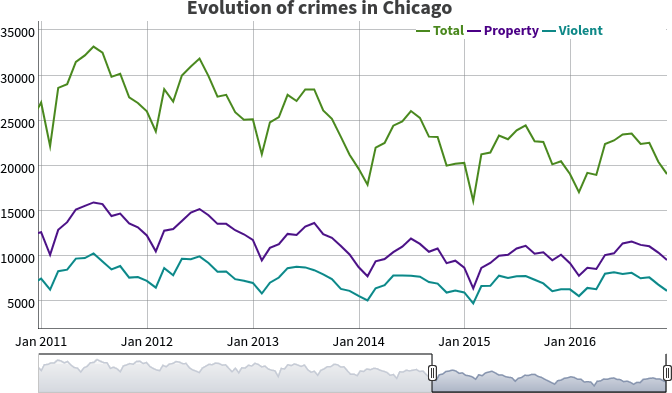
\includegraphics[width=0.8\textwidth]{images/single-chicago}
	\caption{Crime statistics in Chicago between January 2011 and December 2016}
	\label{fig:single-chicago}
\end{figure}

But this is just the analysis of one very specific city. Are more cities experiencing the same decrease in registered crimes? In figure \ref{fig:comp-base} we can see a comparison of four cities: Atlanta, Chicago, Philadelphia, and San Francisco (from the South, Midwest, Northeast, and West regions, respectively).

This time series opens a new picture on our understanding of crime statistics. It is well known that Chicago is particularly exemplary~\cite{Beardsley2014} on the early adoption of RMS systems, leading to an statistically robust data set. But how can we guess if this is the case with other cities? It is quite glaring that total crimes number by themselves are probably not the best number to analyse more than one city at the same time. For this reason we decided to give the user the ability to normalise data using two criteria: (a)~by population, depicted on figure \ref{fig:comp-pop}; and (b)~by crime mean\footnote{These ratios are widely used while comparing crime reports of different cities to study the relative time-evolution of crimes.~\cite{Boba2004}}.

\begin{figure}[H]
	\centering
	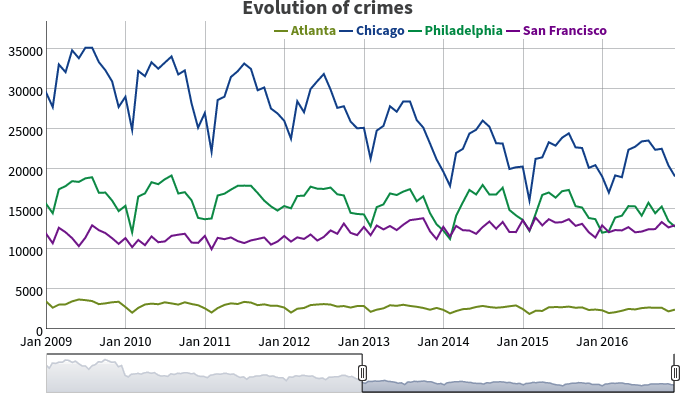
\includegraphics[width=0.8\textwidth]{images/base}
	\caption{Comparison of crime statistics between Atlanta, Chicago, Philadelphia, and San Francisco}
	\label{fig:comp-base}
\end{figure}

% \begin{figure}[H]
% 	\centering
% 	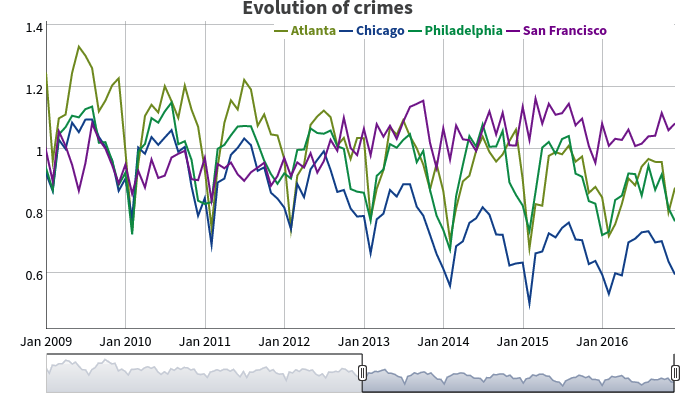
\includegraphics[width=0.8\textwidth]{images/mean}
% 	\caption{Comparison of crime statistics between Atlanta, Chicago, Philadelphia, and San Francisco; normalised by crime mean}
% 	\label{fig:comp-mean}
% \end{figure}

\begin{figure}[H]
	\centering
	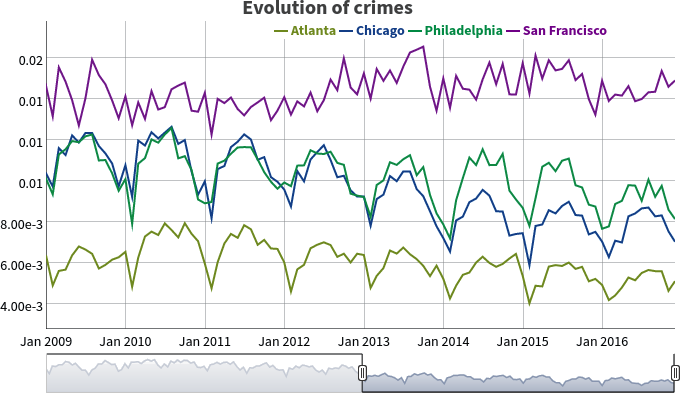
\includegraphics[width=0.8\textwidth]{images/pop}
	\caption{Comparison of crime statistics between Atlanta, Chicago, Philadelphia, and San Francisco; normalised by population}
	\label{fig:comp-pop}
\end{figure}

The differences in the three time series are remarkable. Using normalisation methods give us a much richer approach to do a qualitative comparative analysis. It is remarkable how different the West (San Francisco, Los Angeles, Portland, ...) is from the rest of the US: they are all seem to follow completely different cyclic patterns; crimes are on the rise, whilst the rest of the country seems to be improving their cities in regards to crime statistics.

Again, we could interpret these statistics in many ways. The obvious one seems to be that young and upper-class people, specially because of Hollywood and the Silicon Valley, are moving to the West coast, leading to more opportunities to commit crimes (usually property crimes). But without any proper analysis on the social predictors, this is just a wild conjecture. Quoting Rachel Boba~\cite{Boba2004},
\begin{quotation}
    \emph{All of these types of data serve a purpose in providing a picture of crime. However, depending on which data are used the picture may be very different.}
\end{quotation}


\bigskip
Last but not least, we would like to talk about Seattle (figure \ref{fig:single-seattle}). We included this city as an example of why data scientists and data analysts are required in today's world. When we first saw the data, we were quite shocked. How come there is such a huge gap of data between February 2013 and August 2014?

What we found is that for some reason, they don not have the \emph{Event Clearance Date} for most of the crimes reported in this period, but they do have the \emph{General Offense Number} (in the format \inline{YYYYN}, where \inline{YYYY} is the year \inline{N} seems to be an internal tracking code); this surely could be used by a data scientist to repopulate the missing values using data governance techniques.

\begin{figure}[H]
	\centering
	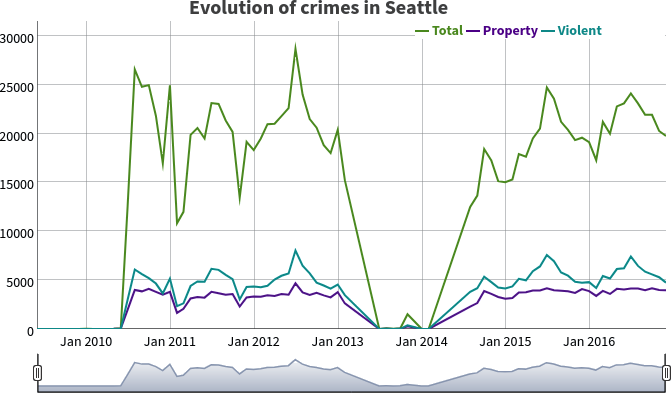
\includegraphics[width=0.8\textwidth]{images/single-seattle}
	\caption{Crime statistics in Seattle between January 2011 and December 2016}
	\label{fig:single-seattle}
\end{figure}
